% !TEX root = ./HY-CS-main.tex
\color{black}
\chapter{Datamalli oppijan kehittymisesta\label{datamallioppijankehittymisesta}}

Oppimisanalytiikassa yhdistelemällä tilastollisia menetelmiä ja predicative modelling käyttämällä voidaan kohdentaa ohjausta opiskelijoiden haasteisiin oppimisessa ja tarjoamalla kohdistettua tukea saatavan datan avulla \citep{ranjeethSurveyPredictiveModels2020}. Käytettävät prediktiiviset mallit voivat olla mitä vain datanlouhinta-, koneoppimis- ja keinotekoisilla menetelmillä.

Yksittäisiä opiskelijoita verrataan prediktiivisen mallin avulla muodostettuihin malleihin, jotka kuvaavat keskimääräistä opiskelijaa \citep{wolffImprovingRetentionPredicting2013}. Esimerkiksi prediktiivisen mallinnuksen avulla voidaan ennustaa esimerkiksi kuinka opiskelija tulee menestymään kurssilla; onko pääsemässä kurssia läpi? Tämä tapahtuu edellä kuvatulla tavalla, ja ennusteen perusteella katsotaan onko opiskelija vaarassa olla läpäisemättä kurssia.

\section{Yleistetty malli}
% Multiple linear regressio \citep{agudo-peregrinaCanWePredict2014} \\
% Linear regression \citep{tempelaarSearchMostInformative2015} \\
% Logistic regression \citep{barberCourseCorrectionUsing2012} \\
% Logistic regression \citep{garmanLogisticApproachPredicting2010} \\
% Naïve Bayes algorithm \citep{barberCourseCorrectionUsing2012} \\
% Decision tree \citep{wolffImprovingRetentionPredicting2013} \\


% Linear regressionista hyvää tietoa \citep{rossIntroductoryStatistics2017} - Ch 12 \\
% Naive Bayessian Ch 16

Ennen datan syöttämistä millekään analysiontia tai luokittelua tekevälle mallille, tulee aineistolle suorittaa esikäsittely \citep{romeroSurveyPreProcessingEducational2014}. Esikäsittelyssä ensin tarvittava data kerätään kasaan ja ryhmitellään sopivasti järkeviin kokonaisuuksiin. Datan ollessa kasassa ryhmiteltynä, poistetaan siitä kaikki epäolennainen ja virheellinen sisältö. Kohdistaaksemme analyysin opiskelijoihin, täytyy aineistosta tunnistetaa käyttäjät sekä heidän eri asiointisessiot. Tämän jälkeen valitaan sopivat selittävät muuttujat jättääksemme kaikki korreloivat ja toisteiset muuttujat pois. Tämän jälkeen isoista data-aineistoista poistetaan aiempien vaiheiden jälkeen turhiksi jääneet kentät, jotka olisivat epäolennaisia prosessille tai toisteisia. Lopuksi tarkastellaan mahdollisuutta muodostaa uusia muuttujia olemassa olevien muuttujien perusteella. Esimerkiksi voidaan normalisoida muuttujan arvot jollekin tietylle välille tai muutetaan esitystapaa sopivammaksi.

Datamallin rakentamisessa on useita vaiheita, ja yleensä puhutaan iteratiivisesta prosessista \citep{hamalainenClassifiersEducationalData2010}. Iteratiivisen prosessin aikana kokeillaan useita erilaisia malleja, datan esitysmuotoja ja algoritmien asetuksia löytääksemme parhaan mahdollisen. Valitun mallin toimivuus voidaan todentaa luokittelun onnistumisella - jos mallille tulee lian monta virhettä, voidaan mallin soveltuvuus kyseenalaistaa.

Oppimisanalytiikassa usein käytetään luokittelua, kuten myös opetuksessa yleisesti opettajien arvioidessa oppijoiden tietotasoa, motivaatiota ja käytöstä \citep{hamalainenClassifiersEducationalData2010}. Oppimisanalytiikassa luokittelua tehdään selitettävän muuttujan arvoa ennustavalla mallilla, joka hyödyntää selittävien muuttujien arvoja. Luokittimia voidaan tehdä joko ammattilaisten käsityönä tai nykyisin yleisemmällä tavalla opettaa luokitin luokittelemaan olemassa olevalla datalla.

Useissa oppimisanalytiikkaa käsitelleissä tutkimuksissa on kokeiltu erilaisia luokittelualgoritmejä data-aineistolle löytääkseen parhaiten toimivan mallin \citep{akcapinarUsingLearningAnalytics2019}. Kokeiltuja algoritmejä ovat naiivi Bayes, Classification Tree, Random Forest, tukivektorikone (SVM), neuroverkko, CN2 rules ja k-lähinaapurimenetelmä. Parhaiten toimivaa mallia voidaan etsiä esimerkiksi suorituskykymittauksin, jossa tarkastellaan tarkkuutta, herkkyyttä, yksityiskohtaisuutta ja F-Measurea.

Yksi tapa toteuttaa malli on käyttää ristivalidointia \citep{deisenrothMathematicsMachineLearning2020}. Yksi tälläinen ristivalidoinnin malli on k-kertainen ristiinvalidointi. Tässä mallissa aineisto jaetaan $k$ osaan, joista yhtä osaa käytetään testiaineistona $\mathcal{V}$ ja $k-1$ osaa koulutusaineistona $\mathcal{R}$. Tällöin käytettävästä koulutusaineistosta käytetään suurin osa mallin kouluttamiseen, mutta samasta aineistosta saadaan myös tarkastusaineisto. Ristiinvalidoinnissa käydään läpi kaikki mahdolliset $k$ vaihtoehtoa valita testausaineisto eli jaetaan data-aineisto kahteen osaan $D = \mathcal{R} \cup \mathcal{V}$, missä $\mathcal{R} \cap \mathcal{V} = \emptyset$. Näiden $k$-suorituskerran muodostamien mallien suorituskyky tarkastellaan keskiarvona.

\begin{figure}[h]
    \centering
    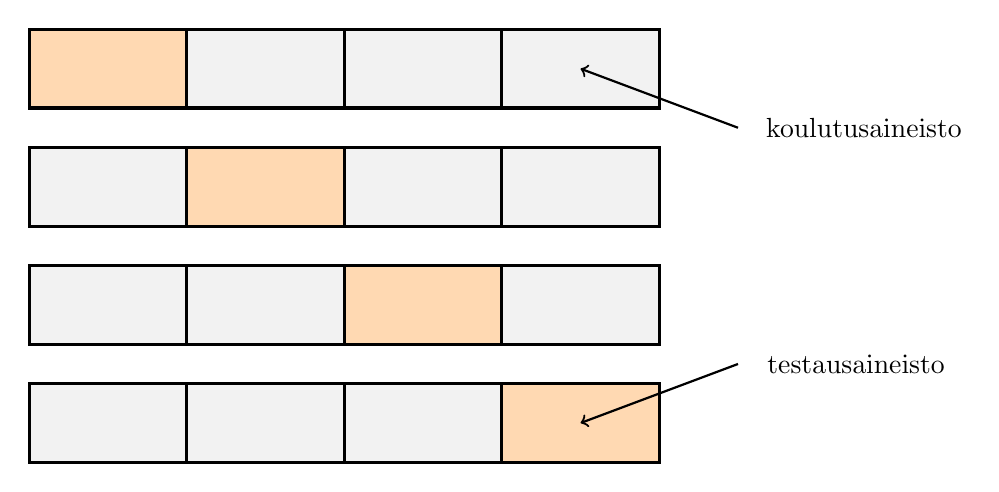
\begin{tikzpicture}
        \filldraw[color=black, fill=black!5, very thick] (0,0) rectangle (2,1);
        \filldraw[color=black, fill=black!5, very thick] (2,0) rectangle (4,1);
        \filldraw[color=black, fill=black!5, very thick] (4,0) rectangle (6,1);
        \filldraw[color=black, fill=orange!30, very thick] (6,0) rectangle (8,1);

        \filldraw[color=black, fill=black!5, very thick] (0,1.5) rectangle (2,2.5);
        \filldraw[color=black, fill=black!5, very thick] (2,1.5) rectangle (4,2.5);
        \filldraw[color=black, fill=orange!30, very thick] (4,1.5) rectangle (6,2.5);
        \filldraw[color=black, fill=black!5, very thick] (6,1.5) rectangle (8,2.5);

        \filldraw[color=black, fill=black!5, very thick] (0,3) rectangle (2,4);
        \filldraw[color=black, fill=orange!30, very thick] (2,3) rectangle (4,4);
        \filldraw[color=black, fill=black!5, very thick] (4,3) rectangle (6,4);
        \filldraw[color=black, fill=black!5, very thick] (6,3) rectangle (8,4);

        \filldraw[color=black, fill=orange!30, very thick] (0,4.5) rectangle (2,5.5);
        \filldraw[color=black, fill=black!5, very thick] (2,4.5) rectangle (4,5.5);
        \filldraw[color=black, fill=black!5, very thick] (4,4.5) rectangle (6,5.5);
        \filldraw[color=black, fill=black!5, very thick] (6,4.5) rectangle (8,5.5);

        \draw[thick, ->] (9,1.25) -- (7,0.5);
        \node[] at (10.5,1.25) {testausaineisto};

        \draw[thick, ->] (9,4.25) -- (7,5);
        \node[] at (10.6,4.25) {koulutusaineisto};
    \end{tikzpicture}
    \caption{Ristiinvalidoinnissa data-aineisto jaetaan $k$-osaan, missä $k-1$ osaa ovat koulutusaineistoa (harmaalla merkityt osuudet) ja yksi osa testausaineistoa (oranssilla merkitty osuus) \citep{deisenrothMathematicsMachineLearning2020}.}
\end{figure}

Mallin kouluttamisen jälkeen koulutusaineistolla $\mathcal{R}$ tarkastellaan koulutetun mallin $f$ suorituskykyä testausaineiston $\mathcal{V}$ avulla \citep{deisenrothMathematicsMachineLearning2020}. Tälle halutaan laskea keskineliövirheen neliöjuuri. Näin toteutettaessa saadaan jokaiselle $k$-osalle toteutettua malli $f^{(k)}$ koulutusaineiston $\mathcal{R}^{(k)}$ avulla. Näiden pohjalta voidaan laskea tarkastusaineiston $\mathcal{V}^{(k)}$ avulla empiirinen riski $R(f^{(k)}, \mathcal{V}^{(k)})$. Tämän avulla ristiinvalidointi pystyy arvioimaan odotetun yleistysvirheen $$\mathds{E}_{\mathcal{V}}[R(f,\mathcal{V})] \approx \frac{1}{K}\sum^{K}_{k=1} R(f^{(k)}, \mathcal{V}^{(k)}).$$ Prosessissa käytettävässä arvioinnissa on kaksi lähdettä, joista toinen on ettei rajatulla koulutusaineistolla välttämättä saada parasta mahdollista $f^{(k)}$ ja toinen on, ettei testausaineistolla saada tarkkaa arviota riskistä $R(f^{(k)}, \mathcal{V}^{(k)})$.

Mallia toteutettaessa on huomioitava myös ylisovittamisen vaara, jotta mallin tarkkuus ei kärsisi \citep{hamalainenClassifiersEducationalData2010}. Ylisovittamisessa malli on sovitettu koulutusaineistoon niin tarkasti, että se huomioi jopa kaikki erikoistapaukset sekä koulutusdatan virheet. Tämä ilmenee yleensä mallin ollessa liian monimutkainen suhteessa käytettävään data-aineiston kokoon. Mallin sovittamisessa on löydettävä sopiva taso, sillä liian yksinkertaisella mallilla se ei pysty välttämättä tulkitsemaan data-aineistoa ja täten malli on alisovitettu; se ei kuvaa todellisuutta tai kuvaa sitä todella vähän.

Yksi tapa tehdä luokittelua on käyttää naiivia Bayesin luokitinta \citep{natinggaDataScienceAlgorithms2018}. Naiivi Bayesin luokitin pohjautuu Bayesin teoreemaan $$P(A | B) = \frac{P(B | A) \cdot P(A)}{P(B)},$$ missä $A$ ja $B$ ovat tapahtumia, $P(A)$ on todennäköisyys tapahtumalle $A$ olla tosi ja $P(A | B)$ on ehdollinen todennäköisyys tapahtumalle $A$ olla tosi, mikäli tapahtuma $B$ on tosi. Naiivissa Bayesin luokittimessa datapisteiden joukolle annetaan luokka, joka on Bayesin teoreeman perusteella todennäköisin. Tämä tapahtuu laskemalla todennäköisyys sille, kuinka todennäköisesti asia A tapahtuu, jos ehto B saa tietyn arvon.

Bayesin teoreemaa voidaan hyödyntää myös useamman probabilistic eventsin tapauksessa, tällöin käytetään laajennettua Bayesin teoreemaa \citep{natinggaDataScienceAlgorithms2018}. Jos määritellään tapahtumat $B_1, \ldots, B_n$ ovat ehdollisesti riippumattomia tapahtumasta $A$. Tällöin Bayesin teoreema voidaan esittää muodossa $$P(A | B_1, \ldots, B_n) = \frac{P(B_1, \ldots, B_n | A) \cdot P(A)}{P(B_1, \ldots, B_n)}.$$ Nämä satunnaismuuttujat voivat olla diskreettejä tai jatkuvia seuraten todennäköisyysjakaumaa, kuten normaalijakaumaa.

Käytettäessä Bayesilaista todennäköisyyttä, pitää huomioida ovatko vertailtavat tapahtumat riippumattomia toisistaan \citep{natinggaDataScienceAlgorithms2018}. Jos vertaillaan esimerkiksi lämpötilaa ja vuodenaikaa keskenään, niin havaitaan näiden välillä olevan riippuvuus: talvella on kylmää ja kesällä lämmintä. Tämä estää Bayesin teoreeman käyttämisen luokittelemiseen. Tällöin data-aineistoa voidaan kuitenkin hyödyntää tekemällä osittaista analyysiä niille tapahtumille, jotka eivät ole riippuvia toisistaan.

\cite{barberCourseCorrectionUsing2012} omassa tutkimuksessaan yrittäessään tunnistaa opiskelijoita, jotka ovat vaarassa saada hylätyn kurssilta, jolle osallistuu. Toisena mallina tutkimuksessa käytettiin naiivia Bayesia ja kymmenkertaista ristivalidointia. Selittäville muuttujille oli annettu eri painoarvoja riippuen kurssin viikosta. Selittävinä muuttujina oli henkilöön liittyviä taustatietoja, suoritettujen opintopisteiden suhde yritettyihin opintopisteisiin sekä toimintaa verkko-oppimisympäristön keskustelualueella. Verrattuna logistiseen regressioon, lisättyjen selittävien muuttujien kanssa nähtiin kurssin viikolla 0 35 \%-yksikön parannus ennustustarkkuudessa datamäärän ollessa pienempi ja eron kaventuessa huomattavasti lähemmäs toisiaan viikolla 3 datamäärän kasvettua, missä logistisella regressiolla keskimäärin 94\% ennustuksista onnistui ja naiivilla Bayesillä 95\% onnistui.

\color{red}
Useiden eri mallien välisessä vertailussa naiivi Bayes oli ennustustamisen osalta paras algoritmi \citep{kotsiantisPREDICTINGSTUDENTSPERFORMANCE2004}.
\color{black}

Toinen mahdollisuus tehdä tilastollista analyysia kerätylle oppimisdatalle on regressioanalyysi \citep{songLearningAnalyticsEducational2018, romeroEducationalDataMining2010, papamitsiouLearningAnalyticsEducational2014}. Regressioanalyysi voidaan tehdä usealla eri tavalla, joita ovat esimerkiksi yksinkertainen lineaarinen regressio, usean selittäjän lineaarinen regressio ja logistinen regressio. Regression avulla voidaan ennustaa kuinka opiskelija tulee menestymään eri selittävien muuttujien vaikutus huomioiden.

Lineaarinen regressio kuvaa selittävän muuttujan ja selitettävän muuttujan yhteyttä toisiinsa \citep{rossIntroductoryStatistics2017}. Yksinkertaisessa lineaarisessa regressiosa selittäviä ja selitettäviä muuttujia on molempia yksi. Yksinkertainen lineaarinen regressio voidaan esittää kaavana $$Y = \alpha + \beta x + e,$$ jossa $x$ kuvaa selittävää muuttujaa ja $y$ kuvaa selitettävää muuttujaa. Parametrit $\alpha$ ja $\beta$ ovat tuntemattomia suureita, estimaattoreita, jotka estimoidaan datan perusteella.  Muuttuja $e$ kuvaa satunnaista virhettä, jolle yleensä tehdään olettamus sen noudattavan normaalijakaumaa odotus arvolla $0$ ja varianssilla $\sigma^2$. Varianssin oletetaan olevan sama riippumatta selittävistä muuttujista $x$.

Parametrien $\alpha$ ja $\beta$ estimointi voidaan tehdä pienimmän neliösumman estimoinnilla \citep{rossIntroductoryStatistics2017}. Käytettäessä pienimmän neliösumman estimointia, halutaan löytää sellaiset arvot estimaateille $\alpha$ ja $\beta$, joilla virheen neliösumma $\sum^n_{i=1} \epsilon^2_i$ on mahdollisimman pieni. Pienimmän neliösumman estimaatit $\hat{\alpha}$ ja $\hat{\beta}$ parametreille $\alpha$ ja $\beta$ saadaan laskettua kaavoista $$\hat{\beta} = \frac{\sum^n_{i=1}(x_i - \overline{x})(Y_i - \overline{Y})}{\sum^n_{i=1}(x_i - \overline{x})^2}$$ ja $$\hat{\alpha} = \overline{Y} - \hat{\beta}\overline{x},$$ missä $\overline{x} = \frac{\sum^n_{i=1}x_i}{n}$ ja $\overline{Y} = \frac{\sum^n_{i=1}Y_i}{n}$.

Estimoidussa regressioviivassa $y = \hat{\alpha} + \hat{\beta}x$ estimaatti $\hat{\alpha}$ kuvaa suoran kulmakerrointa ja estimaatti $\hat{\beta}$ kuvaa suoran vakiota, eli y-akselin kohtaa missä suora leikkaa y-akselin \citep{rossIntroductoryStatistics2017}. Tämän estimoidun regressioviivan avulla voidaan ennustaa selitettävän muuttujan $y$ arvoja käyttäen selittävän muuttujan x arvoja.

Yksinkertainen lineaarinen regressio voidaan laajentaa usean selittäjän lineaariseksi regressioksi, joka kuvaa kuinka useampi selittävä muuttuja $x$ vaikuttaa selitettävään muuttujaan $Y$ \citep{rossIntroductoryStatistics2017}. Matemaattisena kaavana esitettynä tämä olisi $$Y = \beta_0 + \beta_1x_1 + \beta_2x_2 + \ldots + \beta_kx_k + e,$$ jossa $Y$ on selitettävä muuttuja, ja $x_i$ kuvaa selittäviä muuttujia, missä $i = 1, \cdots, k$. Regressioparametrejä yhtälössä kuvaa $\beta_0, \beta_1, \cdots, \beta_k$ ja satunnaisvirhettä $e$.

Kuten naiivin Bayesin osalta, täytyy myös regressiossa välttää sellaisia selittäviä muuttujia, jotka korreloivat keskenään; toisin sanoen näiden arvot ovat riippuvaisia toisistaan eivätkä täten ole riippumattomia \citep{daoudMulticollinearityRegressionAnalysis2017}. Tätä ilmiötä kutsutaan multikollineaarisuudeksi. Ilmiö voidaan havaita tapauksissa, joissa tapahtuu suurta vaihtelua estimoitujen kertoimien osalta lisättäessä tai poistettaessa selittäviä muuttujia tai suurta vaihtelua kertoimissa muutettaessa tai poistettaessa yksittäisiä datapisteitä.

Yhdistelläksemme intervallilla liikkuvia muuttujia kategoristen muuttujien kanssa, kuten onko henkilöllä jokin tietty ominaisuus, voidaan käyttää dummy-muuttujia kuvaamaan näitä arvoja \citep{rossIntroductoryStatistics2017}. Tämän avulla pystytään hyödyntämään sellaisia selittäviä muuttujia, jotka eivät ole lähtökohtaisesti numeerisessa muodossa. Jos esimerkiksi usean selittäjän lineaarisessa regressiossa muuttuja $x_3$ kuvaa onko opiskelija tutkinto-opiskelija, voitaisiin tämä esittää numeraalisessa muodossa seuraavasti: $$x_3 = \begin{cases}1 = \text{opiskelija on tutkinto-opiskelija} \\ 0 = \text{opiskelija ei ole tutkinto-opiskelija}\end{cases}.$$

\cite{agudo-peregrinaCanWePredict2014} käytti tutkimuksessaan usean selittäjän lineaarista regressiota etsiessään eri relaatioita opiskelijan toiminnan verkko-oppimisympäristössä ja akateemisen menestyksen väliltä. Riippumattomia selittäviä muuttujia olivat jokainen eri tyyppinen interaktio verkko-oppimisympäristössä ja riippuvana selittävänä muuttujana akateeminen menestys oli esitetty jokaisen opiskelijan saamana kurssin päättöarvosanana. Tutkimuksessa löydettiin merkittäviä relaatioita eri tyyppisten opiskelijan interaktioiden ja akateemisen menestyksen väliltä.

\color{red}
\section{Yksitäiseen oppijaan kohdennetut ehdotukset}

\begin{enumerate}
    \item arviointi- ja muiden seuraamisperiaatteiden muotoileminen malliksi
    \item kurssiarvosanan ennustaminen kurssin edistyessä
    \item suositeltavat jatkokurssit
    \item Educational Data Mining EMD, ainakin \citep{romeroEducationalDataMining2010}
    \item etiikka?! \citep{kailaEthicalConsiderationsLearning2019}
\end{enumerate}

\section{Ehdotuksien tulkinnan rajoitteet}

\begin{enumerate}
    \item virhearviot
    \item yhden asian tajuamatta jääminen !== huono kurssimenestys
    \item model bias
    \item mallien todennäköisyydet - kuinka todennäköisesti tämä pitää paikkansa. voidaanko 72 prosentin todennäköisyyttä pitää sellaisena, että se toimii luotettavana ohjauksen työkaluna?
\end{enumerate}


tilastollinen malli kuvaa optimia, ja verrataan kuinka data sopii tähän malliin